\documentclass[12pt]{article}
%\usepackage{times}
\usepackage{graphicx}
\usepackage{array}
\usepackage{float}
\usepackage{geometry}
%this is a comment
\title{Design and System Implementation: CommunityConnect}
\author{Kamron Ebrahimi \& Samuel Wilson \& Leif Tsang \\ \& Thomas Korsness  \& Quinton Osborn \\ ebrahimk, wilsosam, tsangl, korsnest, osbornq \\ \scriptsize{Git URL: https://github.com/ebrahimk/CS361-001-W2018/tree/CommunityConnect-Assignment-4/projects/ebrahimk/assignment-4}} 
\date{\today}

\begin{document}

\maketitle

\tableofcontents

\section{\bf UML CLass Diagrams}

%\newgeometry{left=2cm, right=2cm, bottom=1cm}
        \begin{figure}[H]
                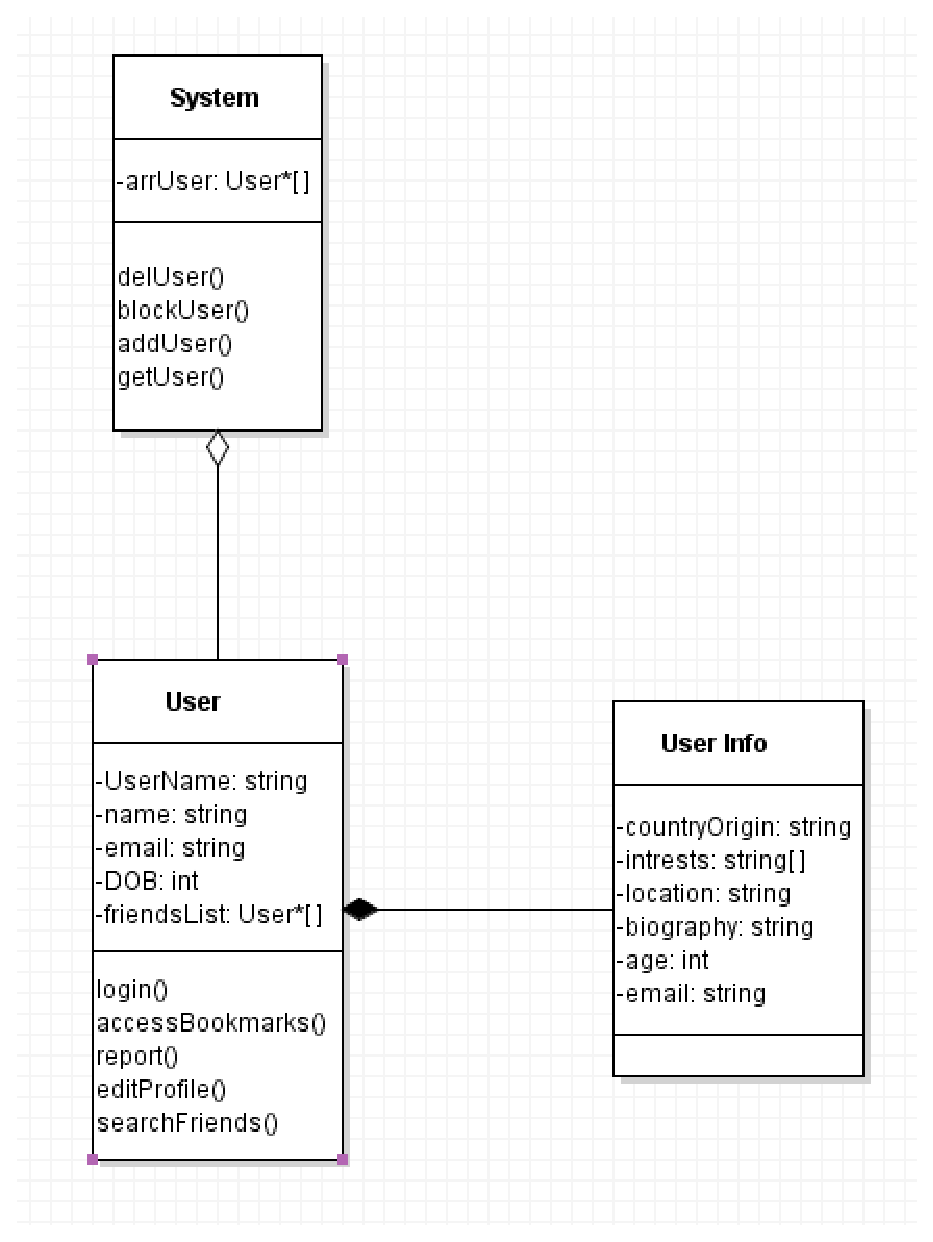
\includegraphics[width =\linewidth,scale=0.5]{classDiagram.eps}
                \caption{Class Diagram 1}
                \label{fig: Class Diagram 1}
        \end{figure}
%\restoregeometry

  \paragraph{\normalfont \indent The CommunityConnect class diagram was simplified and streamlined as the developers gained better insight into what the system architecture will look like. The class diagram is now composed of three classes, a “System” class, which represents the overall back-end data structure in which user profiles are contained, a “User” class, which moderates user access and permissions, providing the CommunityConnnect application with login and authentication features, and a “User Info” class, which contains specific information pertaining to individual users that can be access only upon a successful login. This new design simplifies the CommunityConnect architecture, and removes some unnecessary overhead and abstraction.
  }

\section{\bf Packages}
  \paragraph{\normalfont \indent Looking at the class diagram, we see that there are two main modules: there is the System class, and then the User package that contains the User and User Profile classes. The “System” class on its own is very cohesive, as it handles almost solely things that users interacting with the system are unable to do. Things such as authenticating the user or deleting users should and only are allowed to be performed by the system.
  }
  \paragraph{\normalfont \indent In terms of the “User” package, the cohesion of the User and User Info classes within the package aren’t very high, as we have information between the two that’s pretty similar. For example, the User class has a date of birth attribute, and the User Info class has an age attribute. However, in this case it’s necessary to sacrifice class cohesion for the sake of privacy. When joined into a single package, the cohesion of the package as a whole is higher.
  }
  \paragraph{\normalfont \indent As far as coupling between the User package and System class are concerned, it’s pretty moderate. For example, if we were to modify later what information was contained within the User package, the System class’ data structure would have to be modified in the event that we hard-coded the object’s size.
  }
  \paragraph{\normalfont \indent Coupling will also play a role in each function as we will be authorizing each function to make sure the user can run that command. Authorization should be the same for each function. If some functions were to require a slightly different method of authorization, we could expect to see some issues from this coupling.
  }

\section{\bf Design Patterns}
  \paragraph{\normalfont \indent One of the design patterns we may need to include to implement our system is the Visitor pattern. The User and User Info classes are the first ones that come to mind in considering this. Looking at the UI Prototypes from the SDSUI assignment, it is seen that user profiles will need to be represented in multiple different ways. There’s the full profiles, as well as the profiles seen when browsing connections. There also may be other, smaller ways we use this profile information, such as showing a simplified list of friends that only include their name and picture. The User Information Class would be visited by the System class to serve up profile information for a user whose profile is being visited, and iterate over the elements while selecting the ones that would be needed based on how the profile is being displayed. Another place this would be needed is in our connection algorithm, where the Matches class will need to “visit” the Database class to retrieve a list of users similar to the conditions provided in the search.
  }
  \paragraph{\normalfont \indent Additionally, we may need to include the Builder pattern. The primary purpose for using this design pattern would be in profile creation, as we take a load of information from the user and throw it all into an object to store for access when we want to display profiles later. Also, the User object that contains login information would utilize this design pattern.
  }
  \paragraph{\normalfont \indent Another design pattern that might be included is the Proxy pattern. In order for a user to access the settings on their profile, they need to be authenticated as that user. Thus, access to a specific user’s profile settings needs to be controlled. The Proxy pattern is useful here because we can make a proxy settings object per user that tries to access it and use that to verify that they are authorized to view and modify their settings.
  }

\section{\bf Exceptions and Handling}
  \paragraph{\normalfont \indent Our system doesn’t contain few instances for users to provide free user input, the major exception which we’ll need to handle is a bad login request. In this case, we’ll handle it by asking the user to try to login again, and perhaps remind them that their input is case-sensitive. This login error handling can be directly implemented by the login() method of the “User” class. Also, we can track the number of bad logins and if the user provides five erroneous login attempts in a row, we can store their IP temporarily and block login attempts for an hour, this is feature which the CommunityConnect team decided to add to improve application security.
  }
  \paragraph{\normalfont \indent CommunityConnect’s main purpose is to connect users based off of their ethnic background/interests and their location. Thus the back end searching algorithm needs consistent formatted data to scry through. CommunityConnect would break if users could enter any random string for their location and ethnic background. To handle this Community Connect communicates with a Google maps API when users are setting their location, so the application ensures that users are entering valid locations that can be searched for. Users will also have to choose from a list of countries when entering their country of origin to prevent random user input, that may be erroneous.
  }

\section{\bf Meeting Report}
  \paragraph{\normalfont \indent This week was spent finalizing our plans for tackling CommunityConnects first implementation. The developers now have a solid idea of how to realize the CommunityConnect application. The developers have flushed out all of the classes which will interact within the system, the interface of these class, how these classes will interact and share data with one another, as well as some rough pseudocode for how the methods of each class will be implemented. The CommunityConnect developers now have a host of well organized diagrams and documentation to implement the application.
  }
  \paragraph{\normalfont \indent The team anticipates that next week real, concrete programming will begin starting with the CommunityConnect home page. We want the user to seamlessly interface with the CommunityConnect application, and never feel lost or confused by the flow of events. By the end of next week the team hopes to have all HTML files/ javascript and CSS files completed for a visually engrossing, intuitive user interface.
 } 
  
\begin{center}
\begin{tabular}{ |c|c| }
 \hline
 Kamron Ebrahimi & Meeting Report, LaTex, Slides UI\\
 Quinton Osborn & Packages, Design Patterns, Exceptions/Handling, Slides Design Patters\\
 Leif Tsang & Packages, Class Diagrams, Slides System Design \\
 Thomas Korsness & Class Diagrams, Slides Class Diagram \\
 Samuel Wilson& Slides Planning and Risk Analysis\\
 \hline

\end{tabular}
\end{center}

\end{document}
